\documentclass[11pt,a4paper]{article}
\usepackage[margin=18mm,top=22mm,bottom=20mm]{geometry}
\usepackage{fontspec}\setmainfont{Latin Modern Roman}
\usepackage{amsmath,amssymb,tikz,graphicx,fancyhdr,array,needspace}
\usetikzlibrary{patterns,arrows.meta,decorations.pathmorphing,calc}
\setlength{\headheight}{14pt}
\usetikzlibrary{arrows.meta}
\pagestyle{fancy}\fancyhf{}\renewcommand{\headrulewidth}{0.4pt}
\fancyhead[L]{\textbf{M-08}}\fancyhead[C]{\itshape Fizika (OliyFizika.uz mock test)}\fancyhead[R]{\textbf{Mock №8}}
\fancyfoot[C]{\thepage}
\setlength{\parindent}{0pt}\setlength{\parskip}{3pt}
\newcommand{\opt}[2]{\hspace*{4mm}#1)\ #2\par}
\newcommand{\blank}{\rule{5cm}{0.4pt}}
\begin{document}

\begin{center}{\Large\textbf{FIZIKA}}\end{center}
\noindent\begin{minipage}{\linewidth}
\textbf{1.}\ 10 m/s tezlik bilan vertikal yuqoriga otilgan jism qanday maksimal balandlikka (m) kötariladi? g=10 m/s$^{2}$\par\smallskip
\opt{A}{10}
\opt{B}{20}
\opt{C}{15}
\opt{D}{5}
\end{minipage}\vspace{9pt}\par
\noindent\begin{minipage}{\linewidth}
\textbf{2.}\ Çözib, uzunligi ikki marta oşirilgan prujinaning nisbiy deformatsiya kattaligini aniqlang.\par\smallskip
\opt{A}{1}
\opt{B}{0,5}
\opt{C}{0,6}
\opt{D}{0,2}
\end{minipage}\vspace{9pt}\par
\noindent\begin{minipage}{\linewidth}
\textbf{3.}\ Gorizontal tekislikda arqon yordamida 11 kg massali çana tekis tortib ketilmoqda. Agar arqon gorizont bilan taşkil qilgan burçagining tangensi 0,75 ga teng bölsa, arqonning taranglik kuçini toping (N). Işqalaniş koeffitsiyenti 0,5 ga teng. g=10 N/kg.\par\smallskip
\opt{A}{30}
\opt{B}{20}
\opt{C}{50}
\opt{D}{15}
\end{minipage}\vspace{9pt}\par
\noindent\begin{minipage}{\linewidth}
\textbf{4.}\ Jismning boşlanğiç va oxirgi holatiga boğliq böladigan uçlarga..... kuçlar deyiladi. Nuqtalar örniga töğri javobni qöying.\par\smallskip
\opt{A}{oğirlik}
\opt{B}{musbat}
\opt{C}{potensial yoki konservativ}
\opt{D}{manfiy}
\end{minipage}\vspace{9pt}\par
\noindent\begin{minipage}{\linewidth}
\textbf{5.}\ Qavariq köprikning yuqori nuqtasidan doimiy tezlik bilan ötayotgan 1 t massali maşinaning oğirligi 8 kN ga teng. Unga ta’sir qilayotgan natijaviy kuç (kN) qanday? $g$=10 m/s$^{2}$.\par\smallskip
\opt{A}{2}
\opt{B}{8}
\opt{C}{10}
\opt{D}{18}
\end{minipage}\vspace{9pt}\par
\noindent\begin{minipage}{\linewidth}
\textbf{6.}\ Ikkita toş gorizontga burçak ostida otildi: 1-toş 22,50 burçak ostida 20 m/s boşlanğiç tezlik bilan şimolga, 2-toş esa 45$^\circ$ burçak ostida 10 m/s boşlanğiç tezlik bilan ğarbga. Toşlarning yerga uriliş nuqtalari orasidagi masofani toping (m). g=10 m/s$^{2}$.\par\smallskip
\opt{A}{30}
\opt{B}{40}
\opt{C}{50}
\opt{D}{60}
\end{minipage}\vspace{9pt}\par
\noindent\begin{minipage}{\linewidth}
\textbf{7.}\ Ulkan kema qirğoqqa nisbatan 10 m/s tezlik bilan töğri çiziqli harakatlanmoqda. Uning harakat yönalişida kemaga nisbatan 2 m/s$^{2}$ tezlaniş bilan harakat boşlagan kemadagi odamning qirğoqqa nisbatan harakat tenglamasini (m) toping. $Ox$ öqining musbat yönalişi sifatida kemaning harakat yönalişini tanlab oling.\par\smallskip
\opt{A}{$x = 10 + t^2$}
\opt{B}{$x = 10t - t^2$}
\opt{C}{$x = 10t + t^2$}
\opt{D}{$x = t^2$}
\end{minipage}\vspace{9pt}\par
\noindent\begin{minipage}{\linewidth}
\textbf{8.}\ Balandlikdan gorizontal otilgan jismning normal tezlanişi vaqt ötişi bilan qanday özgaradi?\par\smallskip
\opt{A}{kamayadi}
\opt{B}{ortadi}
\opt{C}{özgarmaydi}
\opt{D}{avval ortadi, keyin kamayadi}
\end{minipage}\vspace{9pt}\par
\noindent\begin{minipage}{\linewidth}
\textbf{9.}\ Qözğalmas blok orqali ötkazilgan ipning bir uçiga 2 kg, ikkinçi uçiga 3 kg massali yuk ilinib tinç holatdan qöyib yuborildi. 3 kg massali jism 2 m pastga tuşganda 2 kg massali jismning kinetik energiyasi (J) qanday böladi? g=10 m/s$^{2}$\par\smallskip
\opt{A}{20}
\opt{B}{12}
\opt{C}{25}
\opt{D}{8}
\end{minipage}\vspace{9pt}\par
\noindent\begin{minipage}{\linewidth}
\textbf{10.}\ 1 kg massali jism gorizontga nisbatan 37$^\circ$ burçak ostida pastga yönalgan 10 N kuç bilan gorizontal sirtda itarib ketilmoqda. Agar jism va sirt orasidagi işqalaniş koeffitsiyenti 0,2 bölsa, jismning tezlanişini (m/s$^{2}$) aniqlang. $g$=10 m/s$^{2}$, sin 37$^\circ$=0,6\par\smallskip
\opt{A}{2,4}
\opt{B}{6}
\opt{C}{3}
\opt{D}{4,8}
\end{minipage}\vspace{9pt}\par
\noindent\begin{minipage}{\linewidth}
\textbf{11.}\ Moddaing massasi 6 marta kamaytirilsa, uning molyar massasi qanday özgaradi?\par\smallskip
\opt{A}{özgarmaydi}
\opt{B}{6 marta ortadi}
\opt{C}{6 marta kamayadi}
\opt{D}{36 marta ortadi}
\end{minipage}\vspace{9pt}\par
\noindent\begin{minipage}{\linewidth}
\textbf{12.}\ Yuzasi 20 cm$^{2}$ bölgan silindrik idiş massasi 7 kg bölgan porşen bilan berkitilgan. Idişdagi gaz temperaturasi 3 marta orttirilganda, porşen dastlabki joyidan qözğalmasligi uçun uning ustiga qanday massali yuk (kg) qöyiş kerak? Atmosfera bosimi 100 kPa ga teng.\par\smallskip
\opt{A}{27}
\opt{B}{36}
\opt{C}{54}
\opt{D}{72}
\end{minipage}\vspace{9pt}\par
\noindent\begin{minipage}{\linewidth}
\textbf{13.}\ Ziçligi $200\ \mathrm{kg/m^3}$ bölgan jism avval benzinga, keyin suvga solindi. Bu jarayonlardagi jismga ta’sir etgan Arximed kuçlarining nisbati $\dfrac{F_{A_1}}{F_{A_2}}$ ni aniqlang. $\rho_{benzin}=700\ \mathrm{kg/m^3}$, $\rho_{suv}=1000\ \mathrm{kg/m^3}$\par\smallskip
\opt{A}{7/10}
\opt{B}{10/7}
\opt{C}{1}
\opt{D}{1/2}
\end{minipage}\vspace{9pt}\par
\noindent\begin{minipage}{\linewidth}
\textbf{14.}\ Kesim yuzi 2,8 mm$^{2}$ bölgan alyuminiy simning uzunligi 1 km. Agar simdan 10 A tok 1 soat mobaynida ötsa, qança issiqlik ajralib çiqadi (MJ)? $\rho$al =2,8$\cdot10^{-8}$ $\Omega$ $\cdot$ m.\par\smallskip
\opt{A}{3,6}
\opt{B}{7,2}
\opt{C}{1,8}
\opt{D}{0,9}
\end{minipage}\vspace{9pt}\par
\noindent\begin{minipage}{\linewidth}
\textbf{15.}\ Elektr lampasi 0,9 kg/m$^{3}$ ziçlikda gaz bilan töldirilgan. Agar lampa yoqilsa, undagi bosim 40 kPa dan 160 kPa gaça ortadi. Bunda lampadagi gaz molekulalarining kvadratik tezligi qanday özgaradi?\par\smallskip
\opt{A}{2 marta kamayadi}
\opt{B}{2 marta ortadi}
\opt{C}{4 marta ortadi}
\opt{D}{4 marta kamayadi}
\end{minipage}\vspace{9pt}\par
\noindent\begin{minipage}{\linewidth}
\textbf{16.}\ Özgaruvçan tok zanjirida tok kuçi $i = 4{,}3\sin(\omega t + \pi/2)$ [mA] qonuniyat bilan tebranmoqda. Tok kuçining $t = T/6$ vaqtdan keyingi oniy qiymatini (mA) aniqlang.\par\smallskip
\opt{A}{4,3}
\opt{B}{2,15}
\opt{C}{1,5}
\opt{D}{3}
\end{minipage}\vspace{9pt}\par
\noindent\begin{minipage}{\linewidth}
\textbf{17.}\ Voltmetrga ketma-ket qilib rezistor ulansa, uning körsatişi qanday özgaradi?\par\smallskip
\opt{A}{ortadi}
\opt{B}{kamayadi}
\opt{C}{özgarmaydi}
\opt{D}{avval ortadi, söng kamayadi}
\end{minipage}\vspace{9pt}\par
\noindent\begin{minipage}{\linewidth}
\textbf{18.}\ Gorizontga burçak ostida otilgan jism harakatida qanday kattalik nolga teng böladi? Havoning qarşilik kuçini hisobga olmang.\par\smallskip
\opt{A}{vertikal tezlaniş}
\opt{B}{eng yuqoridagi tezlik}
\opt{C}{gorizontal tezlaniş}
\opt{D}{yerga urilişdagi tezlik}
\end{minipage}\vspace{9pt}\par
\noindent\begin{minipage}{\linewidth}
\textbf{19.}\ Vakuumli dioddagi töyiniş toki 32 $\mu$A bölsa, katoddan har sekundda neçta elektron uçib çiqadi? e=1,6$\cdot10^{-19}$ C.\par\smallskip
\opt{A}{2$\cdot10^{14}$}
\opt{B}{2$\cdot10^{15}$}
\opt{C}{2$\cdot10^{16}$}
\opt{D}{0,2$\cdot10^{19}$}
\end{minipage}\vspace{9pt}\par
\noindent\begin{minipage}{\linewidth}
\textbf{20.}\ Kondensator plastinkalari orasidagi masofa 10 cm ga teng. Agar qoplamalar orasiga 200 V kuçlaniş berilsa, hosil böladigan maydon kuçlanganligini (kV/m) aniqlang.\par\smallskip
\opt{A}{20}
\opt{B}{0,2}
\opt{C}{2}
\opt{D}{200}
\end{minipage}\vspace{9pt}\par
\noindent\begin{minipage}{\linewidth}
\textbf{21.}\ Fazoning bir nuqtasida janubga tomon 0,3 T, ğarbga 0,9 T va şarqqa 0,5 T magnit induksiya hosil bölmoqda. Şu nuqtadagi natijaviy induksiyani (T) aniqlang.\par\smallskip
\opt{A}{0,8}
\opt{B}{1,1}
\opt{C}{0,5}
\opt{D}{0,7}
\end{minipage}\vspace{9pt}\par
\noindent\begin{minipage}{\linewidth}
\textbf{22.}\ Kondensatordan ötayotgan özgaruvçan tok kuçlaniş tenglamasi U = 100sin50t [V] körinişga ega. Agar kondensatorning siğimi 0,5 mF bölsa, undan ötayotgan tok kuçining amplituda qiymatini toping (A).\par\smallskip
\opt{A}{1}
\opt{B}{0,25}
\opt{C}{25}
\opt{D}{2,5}
\end{minipage}\vspace{9pt}\par
\noindent\begin{minipage}{\linewidth}
\textbf{23.}\ Ötkazgiçda ma’lum bir past haroratda öta ötkazuvçanlik hodisasi yuz berdi. Uşbu past haroratda ötkazgiçning soliştirma qarşiligi qanday özgaradi?\par\smallskip
\opt{A}{tösatdan keskin kamayib, nolga teng bölib qoladi}
\opt{B}{çiziqli tarzda kamayib, 0 K haroratda nolga teng bölib qoladi}
\opt{C}{tösatdan keskin kamayib qoladi}
\opt{D}{egri çiziqli tarzda kamayib, 0 K haroratda nolga teng bölib qoladi}
\end{minipage}\vspace{9pt}\par
\noindent\begin{minipage}{\linewidth}
\textbf{24.}\ Zaryadlangan şarning sirtiy ziçligi 4 nC/m$^{2}$, radiusi 8,85 cm bölsa, şarning sirtidan uning radiusiga teng masofadagi maydon potensialini toping (V). $\varepsilon$=2.\par\smallskip
\opt{A}{5}
\opt{B}{20}
\opt{C}{15}
\opt{D}{10}
\end{minipage}\vspace{9pt}\par
\noindent\begin{minipage}{\linewidth}
\textbf{25.}\ Zaryadlari $-$5e va +3e bölgan suv tomçilari birlaştirilsa, qanday zaryadli tomçi hosil böladi? e – elementar zaryad.\par\smallskip
\opt{A}{$-$2e}
\opt{B}{$-$4e}
\opt{C}{+2e}
\opt{D}{+4e}
\end{minipage}\vspace{9pt}\par
\noindent\begin{minipage}{\linewidth}
\textbf{26.}\ Elektr yoritgiç radiusi 10 cm, yoruğlik kuçi 100 cd bölgan şardan iborat. Manbaning töla yoruğlik oqimini toping (lm).\par\smallskip
\opt{A}{1256}
\opt{B}{1500}
\opt{C}{1700}
\opt{D}{1800}
\end{minipage}\vspace{9pt}\par
\noindent\begin{minipage}{\linewidth}
\textbf{27.}\ Fokus masofasi $-25$ cm bölgan soçuvçi linzaga boş optik öqqa parallel bölgan nur 10 cm li diametr hosil qilib tuşmoqda. Agar nur linzadan ötgaç undan $L$ masofadagi ekranda $300\ \mathrm{cm^2}$ yuzali yoruğ doğ hosil qilayotgan bölsa, $L$ ning qiymatini (cm) aniqlang. $\pi=3$ deb oling.\par\smallskip
\opt{A}{50}
\opt{B}{37,5}
\opt{C}{25}
\opt{D}{75}
\end{minipage}\vspace{9pt}\par
\noindent\begin{minipage}{\linewidth}
\textbf{28.}\ Yoruğlik kuçi 25 cd va 16 cd bölgan ikkita lampa bir-biridan 18 cm masofada turibdi. Ular orasida joylaşgan fotometrik ekranning yoritilganligi bir xil bölişi uçun, ekran birinçi lampadan qança masofada (cm) qöyilişi kerak?\par\smallskip
\opt{A}{12}
\opt{B}{5}
\opt{C}{10}
\opt{D}{15}
\end{minipage}\vspace{9pt}\par
\noindent\begin{minipage}{\linewidth}
\textbf{29.}\ Tinçlikdagi uzunligi 1,6 m bölgan jism yoruğlik tezligiga yaqin bölgan tezlik bilan harakatlanganda, uning uzunligi 32 cm ga özgargan. Jismning tezligi qanday bölgan? $c$ $-$ yoruğlikning vakuumdagi tezligi.\par\smallskip
\opt{A}{0,7$c$}
\opt{B}{0,6$c$}
\opt{C}{0,5$c$}
\opt{D}{0,8$c$}
\end{minipage}\vspace{9pt}\par
\noindent\begin{minipage}{\linewidth}
\textbf{30.}\ Vodorod atomi elektronining 5-energetik sathdagi qiymatini (eV) aniqlang.\par\smallskip
\opt{A}{0,54}
\opt{B}{0,27}
\opt{C}{0,36}
\opt{D}{0,72}
\end{minipage}\vspace{9pt}\par
\noindent\begin{minipage}{\linewidth}
\textbf{31.}\ Agar kumuş atomlarini ionlaş uçun 6,9$\cdot10^{-19}$ J energiya talab qilinsa, uning ionizatsiya potensialini (V) aniqlang.\par\smallskip
\opt{A}{3,7}
\opt{B}{5,1}
\opt{C}{4,3}
\opt{D}{2,9}
\end{minipage}\vspace{9pt}\par
\noindent\begin{minipage}{\linewidth}
\textbf{32.}\ Massasi 1,2 kg bölgan jism gorizontal tekislikda tekislikka parallel bölgan 56 N kuç bilan tortilmoqda. Jism va sirt orasidagi işqalaniş kuçini (N) toping. $\mu$ = 0,8.\par\smallskip
\opt{A}{6,4}
\opt{B}{9,6}
\opt{C}{12}
\opt{D}{2}
\end{minipage}\vspace{9pt}\par
\newpage\noindent\textbf{33–35-test topşiriqlariga mos keluvçi javoblarni (A–F) javob variantlaridan tanlang.}\par\smallskip
Fokus masofasi $F=20$ cm bölgan yiğuvçi linzadan $d=30$ cm masofada balandligi $h=3$ cm bölgan buyum turibdi (rasm).\par\medskip
\begin{center}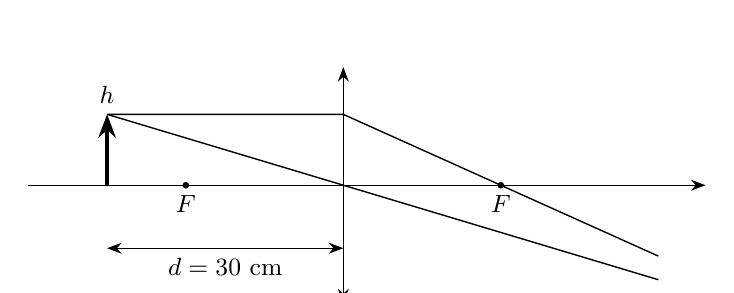
\begin{tikzpicture}[x=1cm,y=1cm,line width=0.5pt,>=Stealth,font=\small]
\draw[->] (-4.0,0)--(4.6,0); \draw[<->] (0,-1.5)--(0,1.5);
\draw[->,very thick] (-3.0,0)--(-3.0,0.9) node[above]{$h$};
\fill (-2.0,0) circle(1.2pt) node[below]{$F$}; \fill (2.0,0) circle(1.2pt) node[below]{$F$};
\draw[<->] (-3.0,-0.8)--(0,-0.8); \node[below] at (-1.5,-0.8) {$d=30\ \mathrm{cm}$};
\draw (-3.0,0.9)--(0,0.9)--(2.0,0)--(4.0,-0.9); \draw (-3.0,0.9)--(4.0,-1.2);
\end{tikzpicture}\end{center}
\noindent\fbox{\begin{minipage}{0.64\linewidth}\vspace{4pt}\textbf{33.}\ Linzadan tasvirgaça bölgan masofani (cm) toping.\\[6pt]\textbf{34.}\ Linzaning çiziqli kattalaştirişini toping.\\[6pt]\textbf{35.}\ Tasvirning balandligini (cm) toping.\vspace{4pt}\end{minipage}\vrule\hspace{6pt}\begin{minipage}{0.28\linewidth}\vspace{4pt}A)\ 2\\B)\ 3\\C)\ 4,5\\D)\ 6\\E)\ 50\\F)\ 60\vspace{4pt}\end{minipage}}\par\vspace{14pt}
\Needspace{9\baselineskip}
\noindent\textbf{36.}\ Qirrasining uzunligi 4 cm bölgan kub şaklidagi 2 ta muz bölagi asosining yuzasi 200 cm$^2$ bölgan, 184,8 g suv quyilgan silindrik idişda taşlandi. $\rho_{muz}=900$ kg/m$^3$.\par\smallskip
\medskip\noindent\textbf{a)\ Muzlar erib ketgandan söng suyuqlikning idiş tubiga beradigan bosimini (Pa) toping.}\par
\noindent\textit{Javob}: a)\ \blank\par
\medskip\noindent\textbf{b)\ Muzlar erib ketgandan söng suyuqlikning idiş tubiga beradigan bosim kuçini (N) hisoblang.}\par
\noindent\textit{Javob}: b)\ \blank\par
\medskip\noindent\textbf{Diqqat!} Javoblaringizni javoblar varaqasiga köçirib yozing.\par\vspace{10pt}
\Needspace{9\baselineskip}
\noindent\textbf{37.}\ Silindrik idişga teng massali suv va kerosin quyildi. Suyuqliklar ustunining umumiy balandligi 45 cm ga teng. $\rho_{kerosin}=800$ kg/m$^3$.\par\smallskip
\medskip\noindent\textbf{a)\ Suv ustunining balandligini (cm) aniqlang.}\par
\noindent\textit{Javob}: a)\ \blank\par
\medskip\noindent\textbf{b)\ Idiş tubidan 20 cm balandlikdagi nuqtada suyuqliklarning hosil qilgan umumiy bosimini (Pa) toping.}\par
\noindent\textit{Javob}: b)\ \blank\par
\medskip\noindent\textbf{Diqqat!} Javoblaringizni javoblar varaqasiga köçirib yozing.\par\vspace{10pt}
\Needspace{9\baselineskip}
\noindent\textbf{38.}\ Uzunligi 25 m, qiyalik burçagi $53^\circ$ bölgan silliq qiya tekislik tepasidan 4 kg massali jism sirpanib tuşdi. $\sin53^\circ=0,8$, $\cos53^\circ=0,6$.\par\smallskip
\medskip\noindent\textbf{a)\ Jismning qiya tekislik etagidagi tezligini (m/s) toping.}\par
\noindent\textit{Javob}: a)\ \blank\par
\medskip\noindent\textbf{b)\ Bu jarayonda oğirlik kuçining bajargan işini (J) toping.}\par
\noindent\textit{Javob}: b)\ \blank\par
\medskip\noindent\textbf{Diqqat!} Javoblaringizni javoblar varaqasiga köçirib yozing.\par\vspace{10pt}
\Needspace{9\baselineskip}
\noindent\textbf{39.}\ Bir atomli ideal gazga 50 J issiqlik berib, hajmi izobarik ravişda 3 marta oşirildi.\par\smallskip
\medskip\noindent\textbf{a)\ Bunda gazning absolyut temperaturasi qanday özgaradi?}\par
\noindent\textit{Javob}: a)\ \blank\par
\medskip\noindent\textbf{b)\ Gazning bajargan işini (J) aniqlang.}\par
\noindent\textit{Javob}: b)\ \blank\par
\medskip\noindent\textbf{Diqqat!} Javoblaringizni javoblar varaqasiga köçirib yozing.\par\vspace{10pt}
\Needspace{9\baselineskip}
\noindent\textbf{40.}\ Issiqlik siğimi 450 J/K bölgan idişda 30 $^\circ$C temperaturali 3 $\ell$ suv bor. Idişga $-12\,^\circ$C temperaturali 1,5 kg muz taşlandi. $c_{suv}=4200$ J/(kg$\cdot$K), $c_{muz}=2100$ J/(kg$\cdot$K), $\lambda_{muz}=330$ kJ/kg.\par\smallskip
\medskip\noindent\textbf{a)\ Natijaviy temperaturani ($^\circ$C) toping.}\par
\noindent\textit{Javob}: a)\ \blank\par
\medskip\noindent\textbf{b)\ Muzning olgan issiqlik miqdorini (kJ) aniqlang.}\par
\noindent\textit{Javob}: b)\ \blank\par
\medskip\noindent\textbf{Diqqat!} Javoblaringizni javoblar varaqasiga köçirib yozing.\par\vspace{10pt}
\Needspace{9\baselineskip}
\noindent\textbf{41.}\ $\alpha$-zarra induksiyasi $B$ bölgan magnit maydonga tik uçib kirdi va $r$ radiusli aylana böylab harakatlana boşladi. $m_\alpha$ — zarraning massasi, $e$ — elementar zaryad.\par\smallskip
\medskip\noindent\textbf{a)\ Uning impulsini aniqlang.}\par
\noindent\textit{Javob}: a)\ \blank\par
\medskip\noindent\textbf{b)\ Kinetik energiyasini aniqlang.}\par
\noindent\textit{Javob}: b)\ \blank\par
\medskip\noindent\textbf{Diqqat!} Javoblaringizni javoblar varaqasiga köçirib yozing.\par\vspace{10pt}
\Needspace{9\baselineskip}
\noindent\textbf{42.}\ Maydon kuçlanganligi $E$ bölgan bir jinsli elektr maydonda harakatlanayotgan proton $l$ masofaga köçib, $A$ nuqtadan $B$ nuqtaga yetib bordi (rasmda $AD\perp \vec E$).\par\smallskip
\begin{center}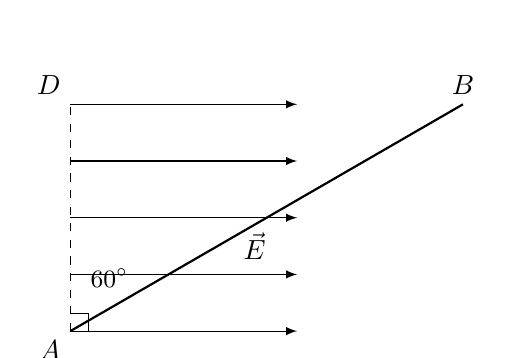
\begin{tikzpicture}[scale=0.9]\foreach \y in {0,0.8,1.6,2.4,3.2}{\draw[-latex] (0,\y)--(3.2,\y);}\draw (0.25,0)--(0.25,0.25)--(0,0.25);\draw[dashed] (0,0)--(0,3.2);\draw[thick] (0,0)--(5.54,3.2);\node[below left] at (0,0) {$A$};\node[above left] at (0,3.2) {$D$};\node[above] at (5.54,3.2) {$B$};\node at (2.6,1.2) {$\vec E$};\node at (0.55,0.75) {\small $60^\circ$};\end{tikzpicture}\end{center}
\medskip\noindent\textbf{a)\ Zarraning kinetik energiyasi qançaga özgarganini aniqlang.}\par
\noindent\textit{Javob}: a)\ \blank\par
\medskip\noindent\textbf{b)\ Zarra $ABDA$ yopiq yöl böylab köçirilganda elektr kuçlar bajaradigan işni aniqlang.}\par
\noindent\textit{Javob}: b)\ \blank\par
\medskip\noindent\textbf{Diqqat!} Javoblaringizni javoblar varaqasiga köçirib yozing.\par\vspace{10pt}
\Needspace{9\baselineskip}
\noindent\textbf{43.}\ Suvdagi nurning intensivligi 24 W/m$^2$ ga teng. $c=3\cdot10^8$ m/s.\par\smallskip
\medskip\noindent\textbf{a)\ Nurdagi elektromagnit maydon energiyasining ziçligini (J/m$^3$) aniqlang.}\par
\noindent\textit{Javob}: a)\ \blank\par
\medskip\noindent\textbf{b)\ Nur suvdagi absolyut qora sirtga tik tuşib töla yutilsa, sirtga beradigan bosimini (Pa) aniqlang.}\par
\noindent\textit{Javob}: b)\ \blank\par
\medskip\noindent\textbf{Diqqat!} Javoblaringizni javoblar varaqasiga köçirib yozing.\par\vspace{10pt}
\Needspace{9\baselineskip}
\noindent\textbf{44.}\ Quyoşning diametri $13,8\cdot10^{8}$ m ga, Yer bilan Quyoşn orasidagi masofa $1,5\cdot10^{11}$ m ga teng. Fokus masofasi 1 m bölgan Yerdagi linza ekranda Quyoşnning haqiqiy tasvirini hosil qilmoqda.\par\smallskip
\medskip\noindent\textbf{a)\ Tasvir bilan linza orasidagi masofani (mm) toping.}\par
\noindent\textit{Javob}: a)\ \blank\par
\medskip\noindent\textbf{b)\ Quyoşn tasvirining diametrini (mm) toping.}\par
\noindent\textit{Javob}: b)\ \blank\par
\medskip\noindent\textbf{Diqqat!} Javoblaringizni javoblar varaqasiga köçirib yozing.\par\vspace{10pt}
\Needspace{9\baselineskip}
\noindent\textbf{45.}\ Ğalayonlangan vodorod atomining ionlaşiş energiyasi 0,85 eV ga teng.\par\smallskip
\medskip\noindent\textbf{a)\ Atom fotonni yutib impuls momentini $1\hbar$ ga oşirsa, uning ionlaniş energiyasi (eV) nimaga teng bölişini aniqlang.}\par
\noindent\textit{Javob}: a)\ \blank\par
\medskip\noindent\textbf{b)\ Atom fotonni yutib impuls momentini $1\hbar$ ga oşirsa, undagi elektronning tezligi neça marta özgarişini aniqlang.}\par
\noindent\textit{Javob}: b)\ \blank\par
\medskip\noindent\textbf{Diqqat!} Javoblaringizni javoblar varaqasiga köçirib yozing.\par\vspace{10pt}
\end{document}